\section*{Appendix}

\subsection*{Setting for Hybrid MILP}

Hybird MILP first call $\alpha,\beta$-Crown with short time-out (TO), then call partial MILP on those inputs which was neither certified nor falsified by this run of $\alpha,\beta$-Crown. We are using two settings of TO, for smaller DNNs we use T0$=10s$, and for the two larger ones, we use TO$=30s$.

The setting for partial MILP for fully-connected DNNs is about how many neurons need to be opened (once set, the selection is automatic). The runtime depending crucially upon the number of open ReLU neurons, we set it quite tightly, only allowing few neuron deviation to accommodate to a particularly accurate/inaccurate bound computation (measure by the weight of the remaining Utility function). As complexity increases with the layer considered, as the size of the MILP model grows, we lower this number with the depth, only committing to an intermediate number for the output neuron (the number of output neurons  is smaller than hidden layer, and this is the most important computation). We experimentally set this number so that each computing the bounds in each hidden layer takes around the same time. Remember that in layer 1, partial MILP is not necessary and propagating bounds using interval arithmetic is already exact. We open [48,48] to compute bounds for hidden layer 2, [21,24] for layer 3, [11,14] for layer 4, [6,9] for layer 5, [3,6] for layer 6, [2,5] for layer 7, [1,4] for hidden layer 8 (if any), and we open [14,17] for the output layer.

For convolutional CNNs, the strategy is adapted, as there is much more neurons, but in a shallower architecture and not fully connected. 
The second layer is computed accurately, opening 200 neurons, which is manageable as there is only one ReLU layer to consider, and accuracy here is crucial.
We do not open any nodes in the third layer (the first fully connected layer) if the output layer is the next one (which is the case for CNN-B-Adv), and instead rely on the choice of important nodes for the output layer. Otherwise, we open 20 neurons.
In the output layer, we open at least 45 neurons (there is less output neurons than nodes in the previous layer), and enlarge the number of open neurons (up to 300) till we find an upper bound, that is a best current MILP solution, of around +0.1 (this 0.1 was experimentally set as target, a good balance between accuracy and efficiency), and compute a guaranteed lower bound (the goal is to guarantee the bound is $>0$).

In Table \ref{table20}, we sum-up the TO and minimum open numbers for each DNN considered.
\begin{table}[h!]
	\centering
	\begin{tabular}{||l||c|c||}
		\hline \hline
		Network & TO for $\alpha,\beta$-Crown  & Minimum number of Open neurons  \\ 		  
		\hline
		MNIST $5 \times 100$ & 10s  & 48,21,11,6,14  \\ \hline
		MNIST $5 \times 200$ & 10s & 48,21,11,6,14  \\ \hline
		MNIST $8 \times 100$ & 10s  & 48,21,11,6,3,2,1,14  \\ \hline
		MNIST $8 \times 200$ & 10s & 48,21,11,6,3,2,1,14  \\ \hline
		MNIST $6 \times 500$ & 30s & 48,21,11,6,3,14 \\ \hline
		CIFAR CNN-B-adv & 30s & 200, 0, 45 \\ \hline \hline
	\end{tabular}
	\caption{Settings of Hybrid MILP for the different {\em hard} instances}
	\label{table20}
	\end{table}


$\alpha,\beta$-Crown uses massively parallel ($>4096$ threads) GPU, while Partial MILP uses 20 CPU-threads.

Notice that a different balance between accuracy and runtime could be set. For instance, we set up the numbers of open neurons to have similar runtime as Refined $\beta$-Crown for the first 4 DNNs ($50s-100s$). We could easily target better accuracy (e.g. for $8 \times 100$ with a relatively high $15\%$ undecided images) by increasing the number of open neurons, with a trade-off on runtime (current runtime is at $61s$).
By comparison, the sweet spot for $\alpha,\beta$-Crown seems to be around TO$=30s$, enlarging the time-out having very little impact on accuracy but large impact on runtime
(see Table \ref{table_beta}).

\medskip
In the following, we provide results comparing $\alpha,\beta$-Crown to other verifiers, to justify our use of $\alpha,\beta$-Crown as state of the art for efficient verifiers as main source of comparison to Hybrid MILP for hard DNN instance.

\newpage 

\subsection*{Comparison $\alpha,\beta$-Crown vs PRIMA}

PRIMA \cite{prima} is a major verifier in the ERAN toolkit. In Table \ref{table9}, we report the comparison between PRIMA and $\alpha,\beta$-Crown, mainly from \cite{crown}. The setting is mainly similar from ours, but numbers are not perfectly comparable as the images tested are not  exactly the same (1000 first or 200 first images for CNN-B-Adv), vs 100 first in Tables \ref{table_hybrid}, \ref{table_beta}. Also, time-out settings and hardware are slightly different. The overall picture is anyway the same.

\begin{table}[h!]
	\centering
	\begin{tabular}{||l||c|c||c||}
		\hline \hline
		Network & $\alpha,\beta$-Crown & Refined $\beta$-Crown & PRIMA \\ 		  
		\hline
		MNIST $5 \times 100$ & N/A  & 14.3\% (102s) & 33.2\% (159s)\\ \hline
		MNIST $5 \times 200$ & N/A & 13.7\% (86s) & 21.1\% (224s) \\ \hline
		MNIST $8 \times 100$ & N/A  & 20.0\% (103s) & 39.2\% (301s)   \\ \hline
		MNIST $8 \times 200$ & N/A & 17.6\% (95s) & 28.7\% (395s)  \\ \hline
		MNIST $6 \times 500$ & 51\% (16s) & $-$ & 64\% (117s) \\ \hline
		CIFAR CNN-B-adv & 18.5\% (32s) & $-$ & 27\% (344s)\\ \hline \hline
		CIFAR ResNet & 0\% (2s) & $-$ & 0\% (2s) \\ \hline \hline
	\end{tabular}
	\caption{Undecided images ($\%$, {\em lower is better}), as computed by $\alpha,\beta$-Crown, Refined $\beta$-Crown, and PRIMA, as reported in \cite{crown}, except for $6 \times 500$ that we run ourselves. N/A means that \cite{crown} did not report the numbers, while $-$ means that Refined $\beta$-Crown cannot be run on these DNNs.}
	\label{table9}
	%\begin{tablenotes}
	%	\footnotesize
%		\item Most data is directly from \cite{crown}. N/A means no data either in \cite{crown} or by our running.
%		\item  $^*$ The data in this row is from our own running on first 100 images of the MNIST dataset.
%		\item  $^{**}$ The data is from \cite{crown} on first 200 images of the CIFAR10 dataset.
%	\end{tablenotes}
	\end{table}

Analysis: On the 4 smallest MNIST networks, PRIMA uses a refined path comparable with Refined $\beta$-Crown. However, it is slower and less accurate than Refined $\beta$-Crown.
On larger {\em hard} networks, PRIMA has also more undecided images than $\alpha,\beta$-Crown, while the runtime is $>5$ times larger.
Hence, Hybrid MILP is more accurate than Prima with similar runtime or faster.

Notice that kPoly \cite{kpoly}, OptC2V \cite{optC2V}, SDP-FO \cite{SDPFI} numbers were also reported in \cite{crown} on these networks, with even more unfavorable results.

\subsection*{Comparison $\alpha,\beta$-Crown vs MN-BaB}

MN-BaB \cite{ferrari2022complete} is an improvement built over PRIMA, using a similar Branch and Bound technique as used in $\alpha,\beta$-Crown. Results in \cite{ferrari2022complete}
are close to those of $\alpha,\beta$-Crown. However, none of the {\em hard} networks from \cite{crown} that we consider have been tested. We thus tested three representative {\em hard} DNNs (first 100 images) to understand how MN-BaB fairs on such hard instances, and report the numbers in Table \ref{table10}. Results are directly comparable with Table \ref{table_hybrid}.


\begin{table}[h!]
	\centering
	\begin{tabular}{||l||c|c||c|c||}
		\hline \hline
		 & $\alpha,\beta$-Crown & $\alpha,\beta$-Crown & MN-BaB & MN-BaB \\ 
		 Network & TO=30s & TO=2000s &  TO=30s & TO=2000s \\ 
		\hline
		MNIST $5 \times 100$ & 55\% (19s) & 50\%(1026s) & 60\% (19s) & 50\% (1027s) \\ \hline
		MNIST $6 \times 500$ & 51\% (16s) & 50\% (1002s) & 58\% (18s) & 55\% (1036s) \\ \hline
		CIFAR CNN-B-adv & 22\% (8.7s) & 20\% (373s) & 43\% (14s) & 24\% (576s) \\ \hline 
	\end{tabular}
	\caption{Undecided images ($\%$, {\em lower is better}), as computed by $\alpha,\beta$-Crown, and MN-BaB}
	\label{table10}
\end{table}

Analysis: results reveal that MN-BaB is slightly slower and slightly less accurate than $\alpha,\beta$-Crown. Notice the specially high number of undecided images for CNN-B-Adv with TO=30s, probably meaning that 30s is too small for MN-BaB on this large DNN.
Hence, Hybrid MILP is more accurate than MN-BaB with similar runtime or faster.

\newpage

	\subsection*{Comparison $\alpha,\beta$-Crown vs NNenum}

NNenum \cite{nnenum} is a complete verifier with good performance according to VNNcomp.
It was the only complete verifier tested in Table \ref{table_complete} to verify more images than $\alpha,\beta$-Crown. The experiments section in \cite{nnenum} does not report
the {\em hard} DNNs we are considering. We tried to experiment it on the same MNIST 
$6 \times 500$ and CIFAR CNN-B-adv as we did in Table \ref{table10} for MN-BaB. Unfortunately, on $6 \times 500$, buffer overflow were reported.
We report in Table \ref{table11} experiments with the same 2000s Time-out (it was $10 000s$ in Table \ref{table_complete})  for a fair comparison with $\alpha,\beta$-Crown, on both 
MNIST $5 \times 100$ and CIFAR CNN-B-Adv. 
On MNIST $5 \times 100$, NNenum is slightly more accurate than $\alpha,\beta$-Crown, but far from the accuracy Hybrid MILP.
On CIFAR CNN-B-adv, NNenum was much less accurate than $\alpha,\beta$-CROWN, and thus of Hybrid MILP. In both test, the runtime of NNenum was also much longer than for Hybrid MILP.


\begin{table}[h!]
	\centering
	\begin{tabular}{||l||c||c||c||c||}
		\hline \hline
		 & $\alpha,\beta$-Crown & NNenum & Hybrid\\ 
		 Network & TO=2000s &  TO=2000s & MILP\\ 
		\hline
		MNIST $5 \times 100$ & 50\%(1026s) & 44\% (1046s) & \bf 13\% (46s)\\ \hline
		CIFAR CNN-B-adv & 20\% (373s) & 40\% (1020s) & \bf 11\% (417s)\\ \hline 
	\end{tabular}
	\caption{Undecided images ($\%$, {\em lower is better}), as computed by $\alpha,\beta$-Crown and NNenum with 2000s time-out, and Hybrid MILP}.
	\label{table11}
\end{table}





\subsection*{Ablation studies}	

In this section, we consider ablation studies to understand how each feature enables the efficiency of pMILP.

\subsubsection*{Time scaling with open nodes}	

First, we explore the time scaling with different number of open nodes, for our full Utility function using nodes in the last two layers (Layer 1 and 2), providing finer details than in Table 3, with the same setting, i.e. previous layer being computing with full MILP.

\begin{table}[h!]
	\centering
	\begin{tabular}{|c|c|c|}
		\hline
		$|X|$ & Time & Uncertainty\\ 
		\hline	0 & 5.9 & 1.702986873\\
		\hline	1 & 9.0 & 1.65469034\\
		\hline	2 & 10.6 & 1.612137282\\
		\hline	3 & 11.6 & 1.571001109\\
		\hline	4 & 12.92 & 1.531925404\\
		\hline	5 & 12.98 & 1.49535638\\
		\hline	6 & 13.6 & 1.46189314\\
		\hline	7 & 14.4 & 1.429953534\\
		\hline max=116 & 3300 & 0.895\\ 
		\hline
		
	\end{tabular}
	\caption{Time scaling with number of nodes. {\bf please complete the table above 7!}}
	\label{table14}
\end{table}


Please make a graph with just this Table. 

		\begin{figure}[h]\hspace*{-0.8cm}
	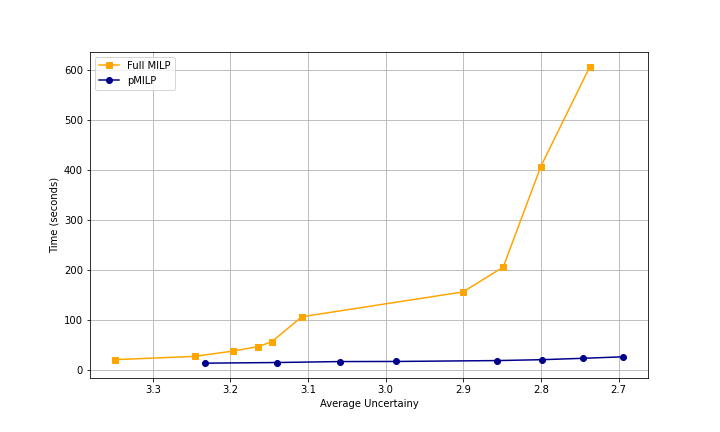
\includegraphics[scale=0.4]{Layer7_comparison_notlog.png}.
	\caption{Plot of time scaling with number of nodes.}
	\label{fig4}
\end{figure}




X axis = accuracy (big to small, can use - accuracy to get that), Y = time.

The exponential complexity with the number of nodes is obvious. 
Computing with $|X| \in$ 21-24, which is what is used by pMILP for this layer, is a good trade off between time and accuracy.

\subsubsection*{Usefulness of computing previous layers accurately}	

Then, we explore the usefulness of computing accurately each layer inductively.
For that, we keep the setting of Table 3 and Table \ref{table14}, but computing the previous layer with LP rather than with full MILP.


\begin{table}[h!]
	\centering
	\begin{tabular}{|c|c|c|}
		\hline
		$|X|$ & Time &  Uncertainty with LP for layer 2 (resp. MILP for layer 2)\\ 
		\hline	5 & 9.3 & 3.247378853 (1.532)\\
		\hline	10 & 10.6 & 3.022145891 (1.371)\\
		\hline	15 & 11.9 & 2.823833569 (1.247)\\
		\hline	20 & 13.1 & 2.638627159 (1.145)\\
		\hline	25 & 16.0 & 2.47324218V (1.061)\\
		\hline	30 & 28.3 & 2.327935601 (0.989)\\
		\hline	35 & 48.1 & 2.195061671 (0.934))\\
		\hline	40 & 89.4 & 2.071075926 (0.921)\\	
		\hline

	\end{tabular}
	\caption{Comparison of accuracy in layer 3 from computing layer 2 inaccurately using LP vs (from computing layer 2 accurately using MILP)}
	\label{table15}
\end{table}
	
This experiment explains the rationale to use divide and conquer protocol, using many calls
(one for each neuron) with relatively small number $|X|$ of open nodes rather than fewer call to MILP with larger number $|X|$ of open nodes. This is clear already with only 1 layer before.


	
%		\begin{figure}[h]\hspace*{-1cm}
%		\includegraphics[scale=0.6]{Layzr3_comparison.png}.
%		\caption{Comparison of layer3 when layer 1 is MILP or LP}
%\label{fig4}
%	\end{figure}




\subsubsection*{restricting open nodes vs time-outs}	

Running full MILP till a small MIP-Gap (typically 0.001) is reached is extremely time inefficient.

Instead, the standard strategy is to set a reasonable time-out and use whatever bound has been generated. We compare this standard strategy with the pMILP strategy of setting a priori a number of open nodes.

Place the two following tables side by side.

% https://tex.stackexchange.com/questions/2832/how-can-i-have-two-tables-side-by-side

ADD THE NUMBER OF NODES FOR pMILP.




\begin{table}[h!]
	\centering
	\begin{tabular}{|c|c|}
	\hline
		Time & Uncertainty\\ 
	\hline	14 & 3.233021901\\
\hline	15.2 & 3.140309921\\
\hline	17.21 & 3.059083103\\
\hline	17.4 & 2.986166762\\
\hline	19.2 & 2.856229765\\
\hline	20.9 & 2.799248232\\
\hline	23.7 & 2.746167245\\
\hline	26.6 & 2.69485246\\	
	\hline
	
	
	\end{tabular}
	\caption{pMILP}
	\label{table12}
	\end{table}
	

	
	\begin{table}[h!]
		\centering
		\begin{tabular}{|c|c|}
			\hline
			Time & Uncertainty\\ 
			\hline	21.1 & 3.348236261\\
			\hline	27.6 & 3.24604282\\
			\hline	38.2 & 3.196640184\\
			\hline	47.1 & 3.164298172\\
			\hline	56.7 & 3.146913614\\
			\hline	106.7 & 3.108035223\\
			\hline	156.3 & 2.900438725\\
			\hline	205.8 & 2.848648426\\	
			\hline	406.7 & 2.800268264 \\	
			\hline	606.1 & 2.737064255\\	
			\hline
			
			
		\end{tabular}
		\caption{full MILP}
		\label{table13}
	\end{table}
	

pMILP obtains 2.8 accuracy in <21 seconds (with 7 open nodes), while full MILP needs 400 seconds to obtain it, a 19x speed up. For 2.7 accuracy, the speedup is $>>$ 22.

This shows that choosing nodes is much more efficient for time/accuracy trade-off than setting time outs and use full MILP. And this is for the smallest DNN we considered (500 hidden neurons, far from the biggest 20k neuron DNN we experimented with)
	
	
	\begin{figure}[h]\hspace*{-0.8cm}
			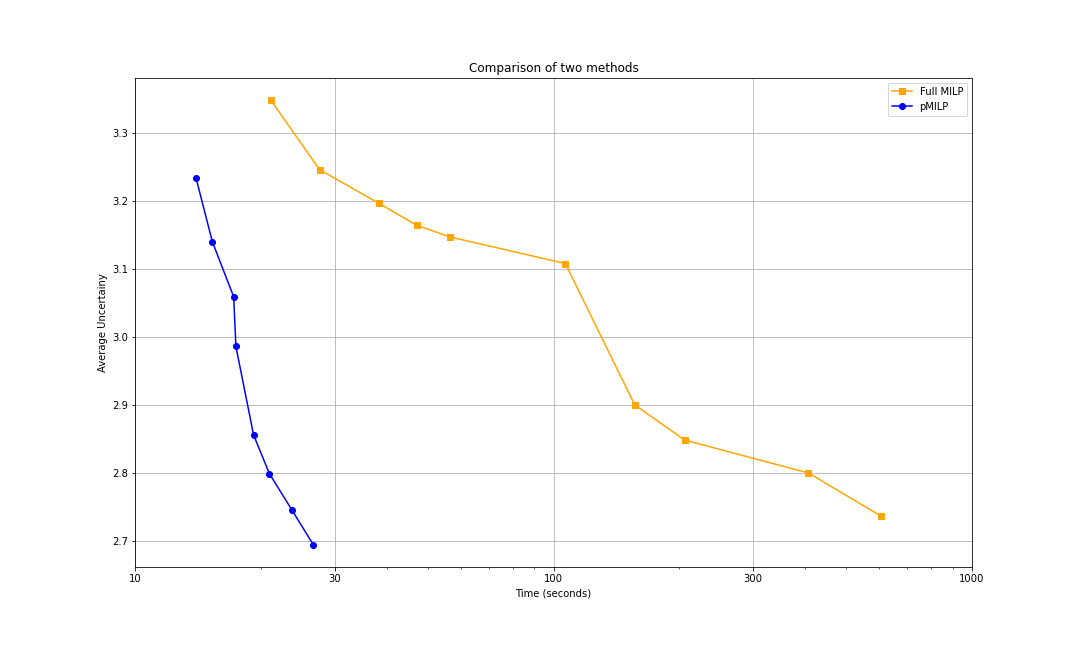
\includegraphics[scale=0.4]{Layer7_comparison.png}.
			\caption{Comparison of uncertainty at layer 7 for full MILP with different time-outs vs pMILP with different number of open nodes}
			\label{fig3}
	\end{figure}
	
	
		\begin{figure}[h]\hspace*{-0.8cm}
		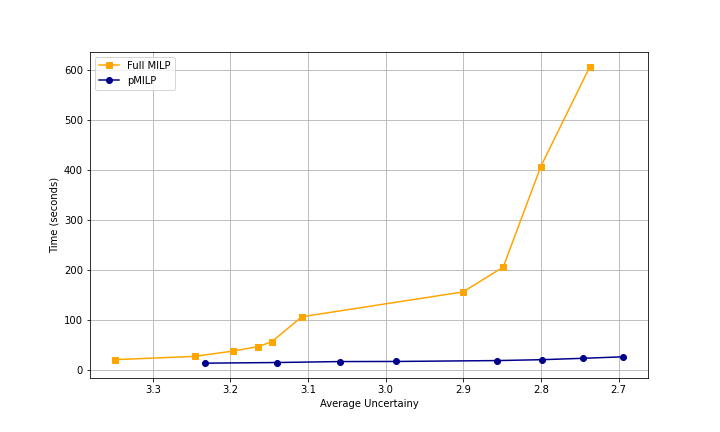
\includegraphics[scale=0.4]{Layer7_comparison_notlog.png}.
		\caption{Comparison of uncertainty at layer 7 for full MILP with different time-outs vs pMILP with different number of open nodes}
		\label{fig5}
	\end{figure}
	
	
Can we have STRAIGHT LINES between points, not this bad connection?

May be log scale for time too.

Also, the caption colors are wrong. You inversed orange and blue.



\begin{align*}
	\Delta(\hat{a}) &= \ReLU(\sol(a))-\sol(\hat{a})\\
	\Delta_0(b) &= \sum_{b} W_{bc}\Delta(\hat{b})\\
	\Delta(c) &= \min(\max((\sol(c)+\Delta_0(c),\LB(c))),\UB(c))-\sol(c)\\
	\Delta(\hat{c}) &=
	\begin{cases}
		\Delta(c)\frac{\LB(c) - \sol(\hat{c})}{\LB(c) - \sol(c)},  &\text{if } \LB(c)< \sol(c) < 0\\
		\Delta(c)\frac{\UB(c) - \sol(\hat{c})}{\UB(c) - \sol(c)},  &\text{if }  0< \sol(c) < \UB(c)\\
		\Delta(c),  &\text{else } 	 
	\end{cases}
\end{align*}